\documentclass[tikz,border=5pt]{standalone}
\usepackage{tikz}
\begin{document}
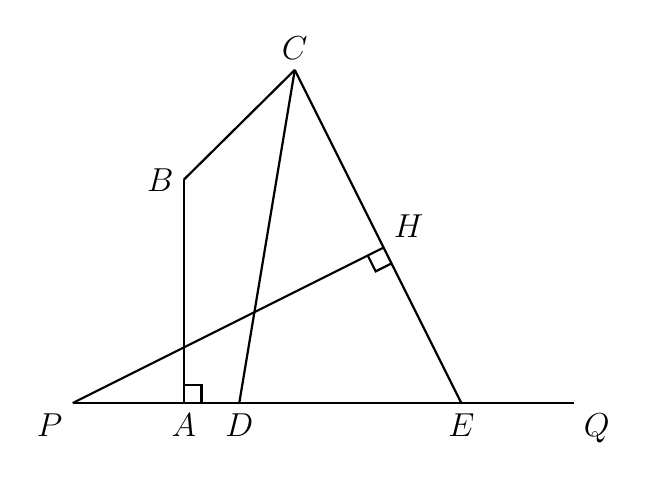
\begin{tikzpicture}[scale=1.5, thick,
  every node/.style={font=\large}]

  % Coordinates (A at origin)
  \coordinate (A) at (0,0);
  \coordinate (P) at (-0.94,0);
  \coordinate (Q) at (3.30,0);
  \coordinate (D) at (0.47,0);
  \coordinate (E) at (2.35,0);
  \coordinate (B) at (0,1.89);
  \coordinate (C) at (0.94,2.82);
  \coordinate (H) at (1.692,1.316);

  % Main line PQ
  \draw (P) -- (Q);

  % Original segments
  \draw (A) -- (B);
  \draw (B) -- (C);
  \draw (C) -- (D);
  \draw (C) -- (E);

  % Perpendicular from P to CE
  \draw (P) -- (H);

  % Right angle mark at A
  \draw (0,0.15) -- (0.15,0.15) -- (0.15,0);

  % Right angle mark at H
  \draw (1.759,1.182) -- (1.625,1.115) -- (1.558,1.249);

  % Labels
  \node[below left] at (P) {$P$};
  \node[below right] at (Q) {$Q$};
  \node[below] at (A) {$A$};
  \node[below] at (D) {$D$};
  \node[below] at (E) {$E$};
  \node[left] at (B) {$B$};
  \node[above] at (C) {$C$};
  \node[above right] at (H) {$H$};

\end{tikzpicture}
\end{document}
